\documentclass[journal,12pt,twocolumn]{IEEEtran}
\usepackage{tikz}
\usepackage{amsmath}
\usepackage{amssymb}
\pagestyle{empty}
\usepackage{setspace}
\singlespacing
\usepackage{caption}
\captionsetup{justification=centering}
\usepackage{amsthm}
\usepackage{amssymb,amsmath}


\begin{document}
\newcommand{\myvec}[1]{\ensuremath{\begin{pmatrix}#1\end{pmatrix}}}
\newcommand{\cmyvec}[1]{\ensuremath{\begin{pmatrix*}[c]#1\end{pmatrix*}}}
\providecommand{\norm}[1]{\lVert#1\rVert}
\newcommand{\mydet}[1]{\ensuremath{\begin{vmatrix}#1\end{vmatrix}}}
\newcommand{\proj}[2]{\textbf{proj}_{\vec{#1}}\vec{#2}}
\newcommand{\abs}[1]{\left\lvert#1\right\rvert}
\newcommand{\RNum}[1]{\uppercase\expandafter{\romannumeral #1\relax}}
\newcommand{\Rnum}[1]{\lowercase\expandafter{\romannumeral #1\relax}}
\let\StandardTheFigure\thefigure
\let\vec\mathbf

\title{
BASICS OF PROGRAMMING

ASSIGNMENT - 1
}
\author{ LAKSHMI GAYATHRI GUDIPUDI - SM21MTECH11001}
\maketitle
\newpage
\bigskip
\renewcommand{\thefigure}{\theenumi}
\bibliographystyle{IEEEtran}
\section*{ Chapter \RNum{2} Ex-\RNum{2} Q.9-\Rnum{2}}
\noindent

Find the Area of Quadrilateral when four points are given
\begin{align}
\vec{P} = \myvec{2\\1}, \vec{Q} =\myvec{3\\5},
\vec{R} =\myvec{-3\\4}, \vec{S} =\myvec{-2\\-2}
\end{align}
\noindent
\section*{\textbf{Solution}}
\noindent
Area of a Quadrilateral PQRS=
\begin{align}
Area (\triangle PQR)+ Area (\triangle PRS)=
\end{align}
\begin{equation}
\frac{1}{2}\norm{(\vec{Q}-\vec{P})\times(\vec{Q}-\vec{R})}+\frac{1}{2}\norm{\mathbf{(\vec{S}-\vec{P})\times(\vec{S}-\vec{R})}}
\label{eq:1}
\end{equation}
For two vectors
\begin{align}
\vec{a}=\myvec{a_1\\a_2} , \vec{b}=\myvec{b_1\\b_2}
\end{align}
\begin{equation}
\norm{\mathbf{\vec{a}\times\vec{b}}}=\abs{(a_1b_2-a_2b_1)}
\label{eq:2}
\end{equation}
\begin{align}
\vec{Q-P}=\myvec{1\\4}\\
\vec{Q-R}=\myvec{6\\1}\\
\vec{S-P}=\myvec{-4\\-3}\\
\vec{S-R}=\myvec{1\\-6}
\end{align}
Using equation \eqref{eq:2}
\begin{equation}
\frac{1}{2}\norm{\mathbf{(\vec{Q}-\vec{P})\times(\vec{Q}-\vec{R})}}
=\frac{1}{2}\abs{(-23)}=11.5
\label{eq:3}
\end{equation}
\begin{equation}
\frac{1}{2}\norm{\mathbf{(\vec{S}-\vec{P})\times(\vec{S}-\vec{R})}}
=\frac{1}{2}\abs{(27)}=13.5    
\label{eq:4}
\end{equation}
Substituting values from equation \eqref{eq:3} and \eqref{eq:4} in equation \eqref{eq:1},We get
\begin{align}
Area =11.5+13.5\\
=25 sq.units
\end{align}
\begin{figure}[!ht]
    \centering
    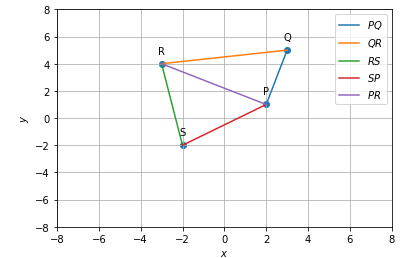
\includegraphics[width=\columnwidth]{QUAD.PNG}
    \caption{Quadrilateral PQRS}
    \label{fig:Quad PQRS}
\end{figure}

\end{document}

